\section{Premissas gerais} \label{section: general settings}
\subsection{Apresentação}
TEXTO A SER ESCRITO NESTA SECAO

\subsection{Premissas}
\begin{enumerate}
	\item O projeto deverá ser desenvolvido por empresa especializada em projetos de engenharia elétrica ou engenheiros eletricistas pleno ou sênior devendo os mesmos comprovar experiência em desenvolvimento de projetos nas áreas solicitadas (administrativas, laboratoriais, ensino, dentre outras) durante o processo licitatório através da certidão de acervo técnico (CAT).
	
	\item O projeto de instalações elétricas obrigatoriamente será desenvolvido para ser construído conforme o cronograma especificado nas premissas básicas da disciplina de arquitetura ou outra em questão, quando estas forem mandatárias.
	
	\item Não havendo disciplina mandatária, a disciplina de elétrica tornar-se-á mandatária e seguirá seu próprio cronograma de desenvolvimento.
	
	\item O projeto será desenvolvido seguindo as etapas estabelecidas no projeto de arquitetura, incluídas as instalações elétricas das edificações propostas no projeto de arquitetura e seu entorno
	
	\item Caso o empreendimento seja dividido em etapas e exista a previsão de uma central de utilidades esta deverá ser prevista e incluída obrigatoriamente na primeira etapa. A central de utilidades (subestação de entrada primária incluída), ramal de entrada vindo da concessionária e ramal(is) de encaminhamento e interligação para a(s)subestação(ões) abaixadora(s) secundárias existentes ou novas, os itens descritos nesta etapa serão elaborados para entrega já na primeira fase do cronograma especificado.
	
	\item A entrega do projeto(desenhos, listagem de materiais, orçamento, caderno de encargos, memorial descritivo, relatórios, cronogramas, dentre outros) seguirá o cronograma de entrega especificado durante a fase licitatória.
	
	\item Caso o projeto seja proposto ou pela contratada ou pela contratante para ser desenvolvido em duas ou mais etapas, os relatórios, projetos, a listagem de materiais, orçamento, o caderno de especificações e cronograma de obra citados no item anterior devem ser entregues de acordo com as etapas propostas e seguindo o cronograma determinado para cada etapa; os documentos serão entregues para serem executados de forma independente de acordo com a etapa a que se referem.
	
	O documento final deverá conter as etapas que poderão ser licitadas e executadas de forma independente;

	\begin{figure}[H]
		\centering
		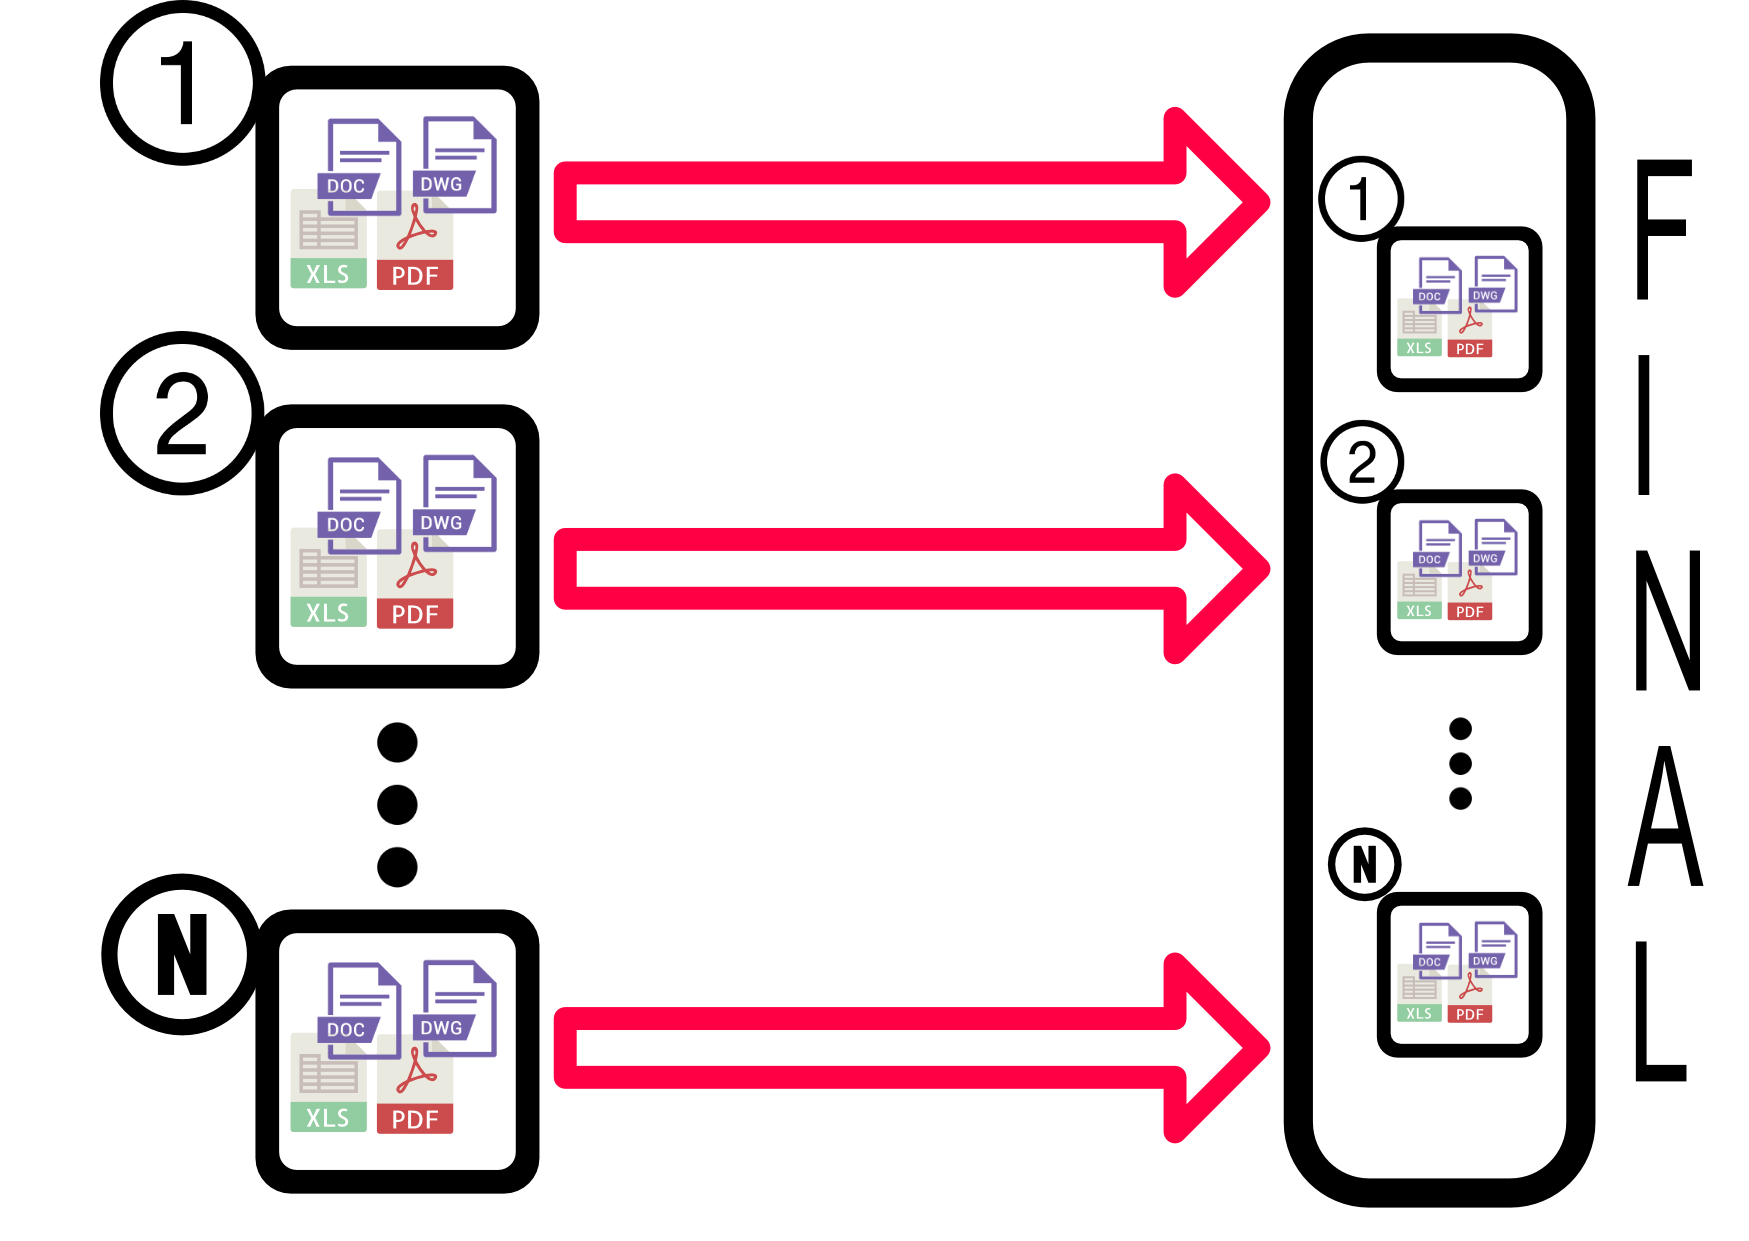
\includegraphics[width=10cm,height=8cm,keepaspectratio]{Figures/2. General Settings/etapas_docs.png}
		\hfill
		\caption{Os documentos e as etapas }
		\label{fig: divisao_etapas}
	\end{figure}
	
	\item O caderno de especificações e o memorial descritivo deverá ser desenvolvido de maneira a contemplar a construção do projeto de acordo com as etapas propostas pela arquitetura, este é um requisito básico a ser considerado durante a entrega final do projeto;
	
	\item O cronograma de obra deverá ser desenvolvido de maneira a contemplar a construção do projeto de acordo com as etapas propostas, este é um requisito básico a ser considerado durante a entrega final do projeto;
	
	\item O orçamento deverá ser desenvolvido de maneira a contemplar a construção do projeto de acordo com as etapas propostas, este é um requisito básico a ser considerado durante a entrega final do projeto;
	
	\item A listagem de materiais deverá ser desenvolvida de maneira a contemplar a construção do projeto de acordo com as etapas propostas, este é um requisito básico a ser considerado durante a entrega final do projeto;
	
	\item Os desenhos a serem entregues deverão ser desenvolvidos de maneira a contemplar a construção do projeto de acordo com as etapas propostas, este é um requisito básico a ser considerado durante a entrega final do projeto;
	
	\item Elementos necessários a uma boa execução de obra que não tenham sido referenciados nos itens acima deverão ser desenvolvidos de maneira a contemplar a construção do projeto de acordo com as etapas propostas, este é um requisito básico a ser considerado durante a entrega final do projeto;
	
	\item Quando o projeto exigir uma subestação de entrada de energia, esta deverá ser construída em local proposto e discutido entre contratante e contratada, observando as características normativas e padrões da concessionária local, com características de tensão e capacidade de suprimento de energia capaz de suprir em condições normais o funcionamento de todas as demandas energéticas elétricas de todo o empreendimento do projeto considerando uma folga mínima para futuras expansões na ordem de 40\% da carga demandada após a conclusão da última etapa; (se aplicável)
	
	\item As subestações abaixadoras devem ser previstas para serem instaladas em áreas externas as edificações as quais servirão. No caso de ser inviável a instalação externa e a mesma necessitar ser instalada no interior da edificação, todos os requisitos de segurança para subestações abrigadas no interior de edificações deverão ser previstos em projetos.
	
	\item Deverá ser considerada uma folga mínima para futuras expansões na ordem de 40\% para as subestações abaixadoras(se aplicável)
	
	\item O projeto poderá compor tensões independentes para o sistema de condicionamento de ar e para as demais distribuições energéticas, objetivando uma maior abrangência de máquinas e equipamentos “padronizados” ofertados no mercado nacional, assim como, vislumbrando uma maior viabilidade técnico-econômica; (se aplicável)
	
	\item O projeto deverá prever uma identificação clara dos sistemas de distribuição, se Normal, se Emergencial ou se Energia Ininterrupta, inclusive com identificações distintas desde sua origem;
	
	\item Um sistema de aterramento em TN-S\footnote{Sistema que separa o neutro da linha da proteção dedicada}, adequado e em características de resistência de aterramento compatível com as normas vigentes, assim como, com as especificidades dos equipamentos a serem instalados;
	
	\item Um sistema de IT-médico com localização de falhas\footnote{Sistema composto por um transformador de separação, anunciador de alarme e localizador de falha de isolamento} em instalações cujos sistemas elétricos relacionados a equipamentos eletromédicos necessitem de atenção especial (se aplicável, de acordo com a norma NBR 13.534/2008); 
	
	\item Um sistema de proteção atmosférica - SPDA compatível com as normas da ABNT, e considerando as características arquitetônicas da edificação, observando as melhores e mais modernas técnicas de construtividade;
	
	\item Um sistema de distribuição que utilize quadros elétricos numa sequência ordenada desde a subestação, ou seja:
		\begin{enumerate}
			\item Quadros gerais normal, emergencial ou ininterrupto na subestação.
			\item Quadros gerais normal, emergencial ou ininterrupto, localizados no pavimento técnico do piso correspondente ao pavilhão, que os alimentarão.
			\item Quadros parciais normal, emergencial ou ininterrupto localizados na entrada de cada um dos Laboratórios.
			\item Quadros parciais normal, emergencial ou ininterrupto localizados em cada área administrativa.
		\end{enumerate}
	
	\item O projeto deverá prever e não poderá deixar de considerar nos sistemas de distribuição, caminhamentos que possuam flexibilidade e possibilitem mais facilidade nas futuras ampliações de carga, utilizando sempre que possível que suas instalações sejam executadas nos pavimentos técnicos e shafts de interligação entre os pavimentos;
	
	\item O projeto deverá prever e não poderá deixar de considerar espaços futuros para instalações de novos disjuntores em quantidade de no mínimo 25 a 30\% do total e suas considerações de cargas, as quais, deverão ser observadas nos dimensionamentos destes quadros; 
	
	\item Deverá atender as exigências do PROCEL;
	
	\item Desenvolvimento de projeto de instalações elétricas compatibilizado com todas as disciplinas;
	
	\item Permitir acessibilidade e facilidade a manutenção e operação posterior do sistema;
\end{enumerate}